\documentclass[12pt,a4paper]{article}
\usepackage[utf8]{inputenc}
\usepackage[T1]{fontenc}
\usepackage{graphicx}
\usepackage{hyperref}
\usepackage{geometry}
\usepackage{setspace}
\usepackage{xcolor}
\usepackage{titlesec}
\usepackage{enumitem}
\usepackage{fancyhdr}
\usepackage{tikz}
\usepackage{tikz-3dplot}
\usetikzlibrary{shapes,arrows,positioning,fit,backgrounds,calc,shadows}
\usepackage{float}

% Layout
\geometry{margin=1in}
\setstretch{1.15}
\pagestyle{fancy}
\fancyhf{}
\rhead{\textbf{November 30 Demo – Architecture}}
\lhead{System Architecture Document}
\rfoot{\thepage}

% Section formatting
\titleformat{\section}{\large\bfseries\color{blue!60!black}}{\thesection.}{1em}{}
\titleformat{\subsection}{\bfseries\color{black}}{\thesubsection}{1em}{}
\titleformat{\subsubsection}{\bfseries\color{teal}}{\thesubsubsection}{1em}{}

\begin{document}

\begin{center}
    \vspace*{0.5cm}
    {\Huge \textbf{Federated ICS Threat Correlation Engine}}\\[0.4cm]
    {\LARGE November 30, 2025 Demo Architecture}\\[0.3cm]
    {\large Version 1.0}\\[0.2cm]
    \textit{Industrial Control Systems Security Team}\\[0.1cm]
    \textbf{Date:} October 14, 2025\\
    \vspace{0.5cm}
\end{center}

\tableofcontents
\newpage

\section{Executive Summary}

This document defines the technical architecture for the November 30, 2025 demonstration of the Federated ICS Threat Correlation Engine.
The focus is on delivering a minimal viable prototype that demonstrates the core value proposition: privacy-preserving collaborative defense through federated learning.

\subsection{Scope}

This architecture document covers the components required for the November 30 demo:

\begin{itemize}[leftmargin=1cm,itemsep=0pt]
    \item 3 simulated facilities with federated learning
    \item Multi-layered detection (LSTM, Isolation Forest, Physics Rules)
    \item Correlation engine for multi-source fusion
    \item Attack prediction using Graph Neural Networks
    \item Web dashboard for visualization
    \item Privacy preservation mechanisms
\end{itemize}


\subsection{Key Architectural Goals}

\begin{enumerate}[leftmargin=1cm,itemsep=0pt]
    \item \textbf{Federated Learning:} 3 facilities learning collaboratively in 6-24 hours
    \item \textbf{Real-Time Detection:} Detect threats within 30 seconds
    \item \textbf{Multi-Source Correlation:} Combine 3 detection methods
    \item \textbf{Attack Prediction:} 67\% accuracy for next-step prediction
    \item \textbf{Privacy-Preserving:} Mathematical guarantees (ε=2.0, δ=10⁻⁵)
    \item \textbf{Demonstrable:} Visual proof through dashboard
\end{enumerate}

\section{System Overview}

\subsection{High-Level Architecture}

The demo system consists of five primary layers:

\begin{figure}[H]
\centering
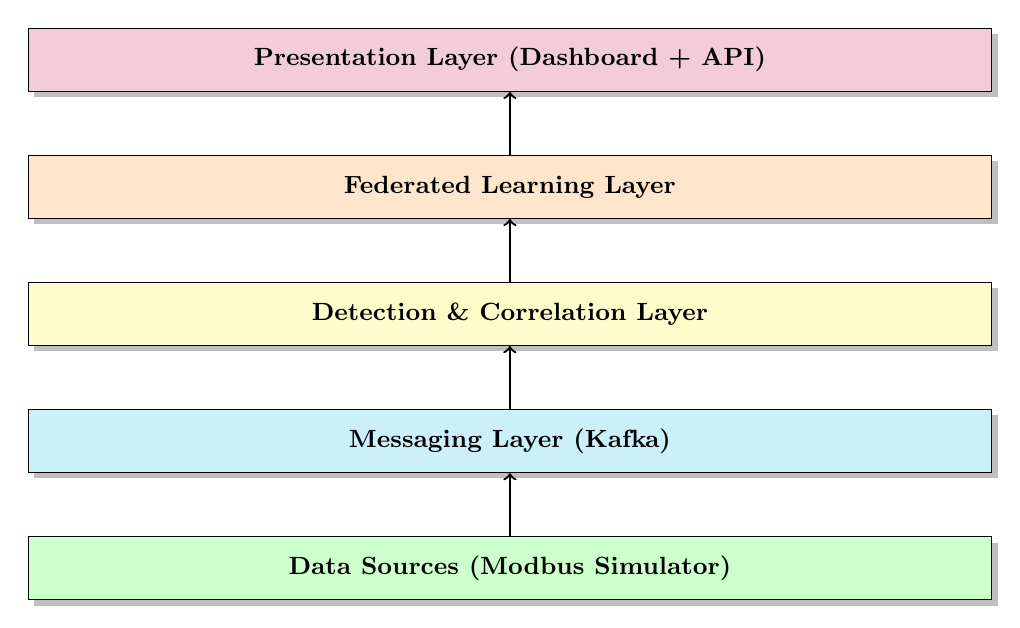
\begin{tikzpicture}[
    node distance=0.8cm,
    layer/.style={rectangle, draw, fill=blue!20, text width=12cm, align=center, minimum height=0.8cm, font=\bfseries\small, drop shadow}
]

\node[layer, fill=purple!20] (api) {Presentation Layer (Dashboard + API)};
\node[layer, below=of api, fill=orange!20] (fl) {Federated Learning Layer};
\node[layer, below=of fl, fill=yellow!20] (detection) {Detection \& Correlation Layer};
\node[layer, below=of detection, fill=cyan!20] (messaging) {Messaging Layer (Kafka)};
\node[layer, below=of messaging, fill=green!20] (sources) {Data Sources (Modbus Simulator)};

\draw[->, thick] (sources) -- (messaging);
\draw[->, thick] (messaging) -- (detection);
\draw[->, thick] (detection) -- (fl);
\draw[->, thick] (fl) -- (api);

\end{tikzpicture}
\caption{Five-Layer Demo Architecture}
\end{figure}


\section{Component Architecture}

\subsection{Layer 1: Data Sources}

\subsubsection{Modbus Simulator}

\textbf{Purpose:} Generate realistic ICS traffic for 3 simulated facilities

\textbf{Technology:} Python 3.11+, pyModbus

\textbf{Responsibilities:}
\begin{itemize}[leftmargin=1cm,itemsep=0pt]
    \item Simulate normal operational data (temperature, pressure, flow)
    \item Generate realistic sensor readings with noise
    \item Support attack injection (sudden spikes, gradual drift)
    \item Publish to Kafka topics per facility
\end{itemize}

\subsection{Layer 2: Messaging Layer}

\subsubsection{Apache Kafka}

\textbf{Purpose:} Message bus for decoupled communication

\textbf{Technology:} Apache Kafka 3.x

\textbf{Key Topics:}
\begin{itemize}[leftmargin=1cm,itemsep=0pt]
    \item Sensor data topics (per facility)
    \item Alert topics (per detector)
    \item Unified alerts
    \item FL round notifications
\end{itemize}

\subsection{Layer 3: Detection \& Correlation Layer}

\subsubsection{LSTM Autoencoder}

\textbf{Purpose:} Detect behavioral anomalies in time-series data

\textbf{Technology:} Python 3.11+, TensorFlow 2.x

\textbf{Architecture:}
\begin{itemize}[leftmargin=1cm,itemsep=0pt]
    \item Input: 60-second sliding window (60 timesteps × 10 features)
    \item Encoder: LSTM(128) → LSTM(64)
    \item Latent: Dense(64)
    \item Decoder: LSTM(64) → LSTM(128)
    \item Output: Reconstructed sequence
\end{itemize}

\textbf{Responsibilities:}
\begin{itemize}[leftmargin=1cm,itemsep=0pt]
    \item Subscribe to sensor data from Kafka
    \item Create sliding windows
    \item Compute reconstruction error
    \item Publish alerts when threshold exceeded
\end{itemize}

\textbf{Federated:} Yes - Model weights shared via FL


\subsubsection{Isolation Forest}

\textbf{Purpose:} Detect point anomalies (sudden outliers)

\textbf{Technology:} Python 3.11+, scikit-learn

\textbf{Responsibilities:}
\begin{itemize}[leftmargin=1cm,itemsep=0pt]
    \item Subscribe to sensor data from Kafka
    \item Compute anomaly scores
    \item Publish alerts when threshold exceeded
\end{itemize}

\textbf{Federated:} Yes - Ensemble shared via FL

\subsubsection{Physics Rules Engine}

\textbf{Purpose:} Validate process physics constraints

\textbf{Technology:} Python 3.11+, custom rule engine

\textbf{Rule Types:}
\begin{itemize}[leftmargin=1cm,itemsep=0pt]
    \item \textbf{Range:} value $\in$ [min, max]
    \item \textbf{Rate:} $|\Delta value / \Delta time| <$ max\_rate
    \item \textbf{Dependency:} if A then B must be true
\end{itemize}

\textbf{Responsibilities:}
\begin{itemize}[leftmargin=1cm,itemsep=0pt]
    \item Subscribe to sensor data from Kafka
    \item Evaluate rules against each reading
    \item Publish violations
\end{itemize}

\textbf{Federated:} No - Rules are facility-specific

\subsubsection{Correlation Engine}

\textbf{Purpose:} Combine signals from multiple detection sources

\textbf{Technology:} Python 3.11+, custom correlation logic

\textbf{Architecture:}

\begin{figure}[H]
\centering
\begin{tikzpicture}[
    node distance=1cm,
    source/.style={rectangle, draw, fill=yellow!20, text width=2cm, align=center, minimum height=0.7cm, font=\scriptsize},
    engine/.style={rectangle, draw, fill=orange!20, text width=3cm, align=center, minimum height=1.5cm, font=\small},
    output/.style={rectangle, draw, fill=green!20, text width=2.5cm, align=center, minimum height=0.7cm, font=\scriptsize}
]

\node[source] (lstm) {LSTM\\Anomalies};
\node[source, below=0.5cm of lstm] (if) {Isolation\\Forest};
\node[source, below=0.5cm of if] (physics) {Physics\\Violations};

\node[engine, right=2cm of if] (corr) {Correlation\\Engine\\\\Temporal\\Spatial\\Severity};

\node[output, right=2cm of corr] (alert) {Unified\\Alert};

\draw[->, thick] (lstm) -- (corr);
\draw[->, thick] (if) -- (corr);
\draw[->, thick] (physics) -- (corr);
\draw[->, thick] (corr) -- (alert);

\end{tikzpicture}
\caption{Correlation Engine Architecture}
\end{figure}

\textbf{Responsibilities:}
\begin{itemize}[leftmargin=1cm,itemsep=0pt]
    \item Subscribe to all alert topics
    \item Temporal correlation: events within time window
    \item Spatial correlation: events on same asset
    \item Confidence scoring based on source agreement
    \item Severity assignment
    \item Publish unified alerts
\end{itemize}


\subsection{Layer 4: Federated Learning Layer}

\subsubsection{FL Client}

\textbf{Purpose:} Manage local training and weight transmission

\textbf{Technology:} Python 3.11+, Flower (flwr), TensorFlow/PyTorch

\textbf{Responsibilities:}
\begin{itemize}[leftmargin=1cm,itemsep=0pt]
    \item Receive global model from FL server
    \item Train on local data
    \item Compute weight updates
    \item Apply gradient clipping
    \item Add differential privacy noise
    \item Send weights to FL server
    \item Deploy updated global model
\end{itemize}

\textbf{Deployment:} One FL client per facility (3 total)

\subsubsection{FL Server}

\textbf{Purpose:} Coordinate federated learning rounds

\textbf{Technology:} Python 3.11+, Flower (flwr)

\textbf{Responsibilities:}
\begin{itemize}[leftmargin=1cm,itemsep=0pt]
    \item Schedule FL rounds (every 6 hours)
    \item Distribute global model to clients
    \item Collect weight updates from clients
    \item Apply Byzantine-robust aggregation
    \item Compute new global model
    \item Distribute updated model
    \item Log metrics and status
\end{itemize}

\textbf{Deployment:} Single FL server

\subsubsection{Privacy Engine}

\textbf{Purpose:} Apply differential privacy to weight updates

\textbf{Technology:} Python 3.11+, Opacus (PyTorch) or TensorFlow Privacy

\textbf{Privacy Parameters:}
\begin{itemize}[leftmargin=1cm,itemsep=0pt]
    \item Epsilon (ε): 2.0
    \item Delta (δ): $10^{-5}$
    \item Noise mechanism: Gaussian
    \item Gradient clipping: L2 norm
\end{itemize}

\textbf{Responsibilities:}
\begin{itemize}[leftmargin=1cm,itemsep=0pt]
    \item Generate calibrated noise
    \item Add noise to gradients before aggregation
    \item Track privacy budget
    \item Provide privacy guarantees
\end{itemize}


\subsection{Layer 5: Presentation Layer}

\subsubsection{REST API}

\textbf{Purpose:} Provide HTTP endpoints for dashboard

\textbf{Technology:} Python 3.11+, FastAPI

\textbf{Key Endpoints:}
\begin{itemize}[leftmargin=1cm,itemsep=0pt]
    \item List recent alerts
    \item List facility status
    \item FL round status
    \item FL performance metrics
    \item Inject test attack
\end{itemize}

\textbf{Features:}
\begin{itemize}[leftmargin=1cm,itemsep=0pt]
    \item OpenAPI/Swagger documentation
    \item CORS enabled for dashboard
    \item JSON responses
\end{itemize}

\subsubsection{WebSocket Service}

\textbf{Purpose:} Real-time updates to dashboard

\textbf{Technology:} Python 3.11+, FastAPI WebSockets

\textbf{Events:}
\begin{itemize}[leftmargin=1cm,itemsep=0pt]
    \item New alert detected
    \item FL round initiated
    \item FL round finished
    \item Facility status change
\end{itemize}

\subsubsection{Web Dashboard}

\textbf{Purpose:} Visual interface for demo

\textbf{Technology:} React, TypeScript, Material-UI

\textbf{Pages:}
\begin{itemize}[leftmargin=1cm,itemsep=0pt]
    \item \textbf{System Overview} - 3 facilities with status indicators
    \item \textbf{Alerts Dashboard} - Real-time alert feed
    \item \textbf{FL Status} - Current round, client status, metrics
\end{itemize}

\textbf{Features:}
\begin{itemize}[leftmargin=1cm,itemsep=0pt]
    \item Real-time updates via WebSocket
    \item Color-coded status indicators
    \item Alert details with source breakdown
    \item FL round progress visualization
\end{itemize}


\section{Attack Prediction Component}

\subsection{Neo4j Graph Database}

\textbf{Purpose:} Store MITRE ATT\&CK for ICS knowledge graph

\textbf{Technology:} Neo4j 5.x

\textbf{Data:}
\begin{itemize}[leftmargin=1cm,itemsep=0pt]
    \item MITRE ATT\&CK for ICS techniques
    \item Common attack chains
    \item Historical attack sequences
\end{itemize}

\subsection{Graph Neural Network (GAT)}

\textbf{Purpose:} Predict next attack steps

\textbf{Technology:} Python 3.11+, PyTorch, PyTorch Geometric

\textbf{Architecture:}
\begin{itemize}[leftmargin=1cm,itemsep=0pt]
    \item Input: Current attack state (one-hot encoded technique)
    \item GAT Layer 1: 4 attention heads, 64 dimensions
    \item GAT Layer 2: 4 attention heads, 32 dimensions
    \item Dense + Softmax: Output probability distribution
\end{itemize}

\textbf{Responsibilities:}
\begin{itemize}[leftmargin=1cm,itemsep=0pt]
    \item Load attack graph from Neo4j
    \item Encode current attack state
    \item Predict next techniques with probabilities
    \item Return top-3 predictions
    \item Update graph with new attack chains
\end{itemize}

\textbf{Training:}
\begin{itemize}[leftmargin=1cm,itemsep=0pt]
    \item Pre-trained on historical attack sequences
    \item Fine-tuned during FL rounds
    \item Learns new attack patterns from all facilities
\end{itemize}

\textbf{Federated:} Yes - GNN weights shared via FL

\section{Storage Components}

\subsection{PostgreSQL}

\textbf{Purpose:} Store structured data

\textbf{Technology:} PostgreSQL 15+

\textbf{Stores:}
\begin{itemize}[leftmargin=1cm,itemsep=0pt]
    \item Alerts with metadata
    \item Facility configuration
    \item FL round history
    \item Performance metrics
\end{itemize}

\subsection{Apache IoTDB}

\textbf{Purpose:} Store time-series sensor data

\textbf{Technology:} Apache IoTDB 1.x

\textbf{Stores:}
\begin{itemize}[leftmargin=1cm,itemsep=0pt]
    \item Sensor readings per facility
    \item Temperature, pressure, flow measurements
    \item Historical time-series data
\end{itemize}


\section{Data Flow}

\subsection{Normal Operation Flow}

\begin{enumerate}[leftmargin=1cm,itemsep=0pt]
    \item Modbus simulator generates sensor data
    \item Data published to Kafka topics (per facility)
    \item Detection components consume from Kafka:
    \begin{itemize}
        \item LSTM Autoencoder analyzes sequences
        \item Isolation Forest analyzes points
        \item Physics Rules validate constraints
    \end{itemize}
    \item Each detector publishes alerts to Kafka
    \item Correlation engine consumes all alert topics
    \item Unified alerts published
    \item Alerts stored in PostgreSQL
    \item WebSocket pushes alerts to dashboard
    \item Dashboard displays real-time alerts
\end{enumerate}

\subsection{Federated Learning Flow}

\begin{enumerate}[leftmargin=1cm,itemsep=0pt]
    \item FL Server schedules round (every 6 hours)
    \item Server publishes round notification to Kafka
    \item FL Clients receive notification
    \item Server sends current global model to clients
    \item Each client:
    \begin{itemize}
        \item Loads local training data
        \item Trains model locally
        \item Computes weight updates
        \item Applies gradient clipping
        \item Adds differential privacy noise
        \item Sends weights to server
    \end{itemize}
    \item Server collects all weight updates
    \item Server applies Byzantine-robust aggregation
    \item Server computes new global model
    \item Server distributes updated model to clients
    \item Clients deploy new model for inference
    \item Metrics logged to PostgreSQL
\end{enumerate}

\subsection{Attack Prediction Flow}

\begin{enumerate}[leftmargin=1cm,itemsep=0pt]
    \item Correlation engine detects attack
    \item Attack technique mapped to MITRE ATT\&CK ID
    \item GNN service receives current technique
    \item GNN loads attack graph from Neo4j
    \item Current state encoded as node features
    \item GNN predicts next techniques with probabilities
    \item Top-3 predictions returned
    \item Predictions published to Kafka
    \item Dashboard displays predicted attack path
    \item System increases monitoring on predicted targets
\end{enumerate}


\section{Deployment Architecture}

\subsection{Docker Compose Setup}

All components deployed using Docker Compose.

\textbf{Services:}
\begin{itemize}[leftmargin=1cm,itemsep=0pt]
    \item \texttt{kafka} - Message broker
    \item \texttt{postgres} - Relational database
    \item \texttt{iotdb} - Time-series database
    \item \texttt{neo4j} - Graph database
    \item \texttt{modbus-sim} - Modbus simulator
    \item \texttt{lstm-detector} - LSTM detection service
    \item \texttt{if-detector} - Isolation Forest service
    \item \texttt{physics-detector} - Physics rules service
    \item \texttt{correlation-engine} - Correlation service
    \item \texttt{gnn-predictor} - Attack prediction service
    \item \texttt{fl-server} - FL coordination server
    \item \texttt{fl-client-a} - Facility A FL client
    \item \texttt{fl-client-b} - Facility B FL client
    \item \texttt{fl-client-c} - Facility C FL client
    \item \texttt{api} - REST API service
    \item \texttt{dashboard} - Web dashboard
\end{itemize}

\textbf{Total: 16 containers}


\subsection{Enhanced Network Architecture}

\begin{figure}[H]
\centering
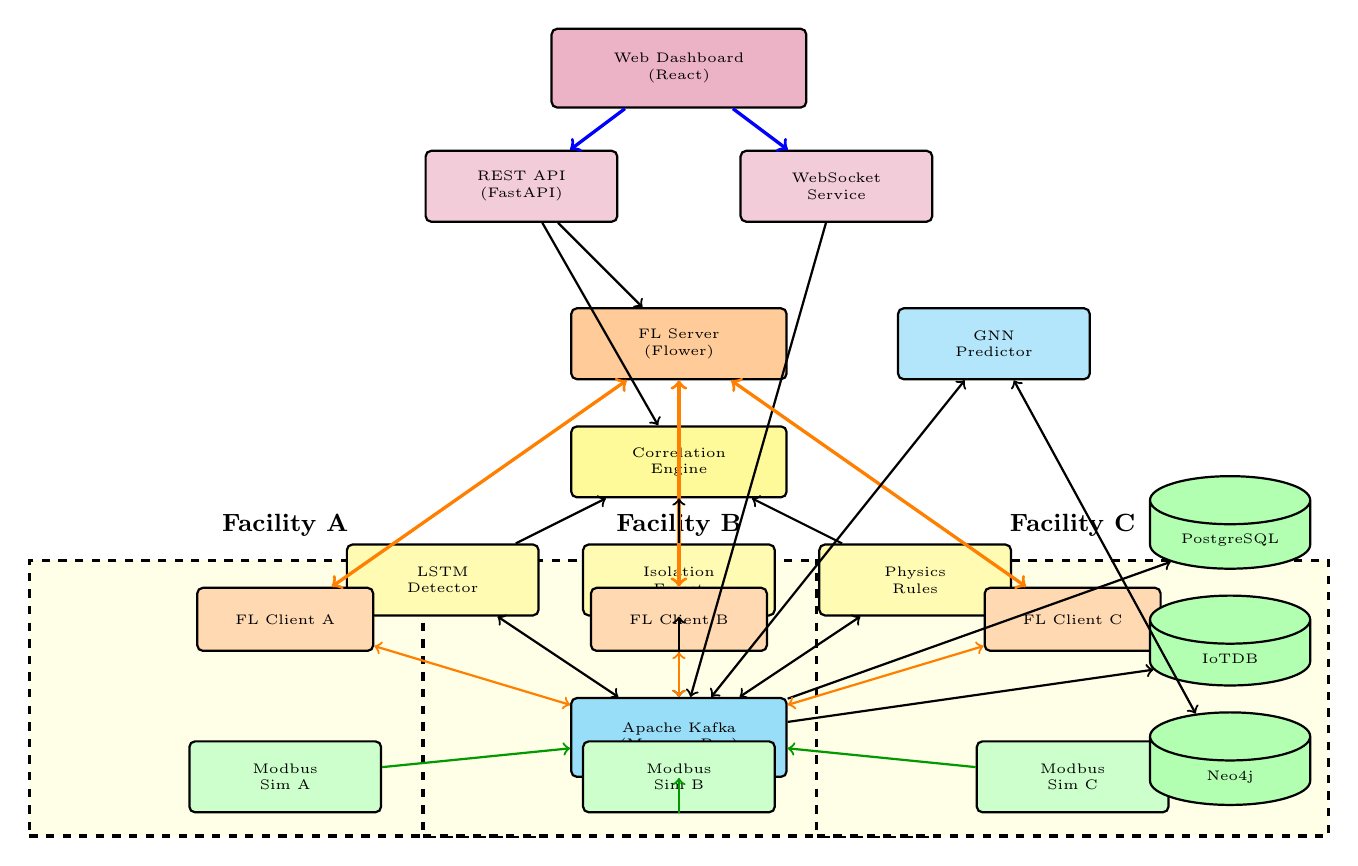
\begin{tikzpicture}[
    node distance=1.2cm and 1.5cm,
    service/.style={rectangle, draw=black, thick, fill=blue!20, text width=2.2cm, align=center, minimum height=0.9cm, font=\tiny, rounded corners=2pt},
    db/.style={cylinder, draw=black, thick, fill=green!30, text width=1.8cm, align=center, minimum height=1cm, font=\tiny, shape border rotate=90, aspect=0.3},
    client/.style={rectangle, draw=black, thick, fill=orange!30, text width=2cm, align=center, minimum height=0.8cm, font=\tiny, rounded corners=2pt},
    facility/.style={rectangle, draw=black, very thick, dashed, fill=yellow!10, minimum width=7cm, minimum height=4cm},
    layer/.style={rectangle, draw=gray, thick, dashed, fill=gray!5}
]

% Facility boxes
\node[facility, minimum width=6.5cm, minimum height=3.5cm] at (-5, -6) {};
\node[facility, minimum width=6.5cm, minimum height=3.5cm] at (0, -6) {};
\node[facility, minimum width=6.5cm, minimum height=3.5cm] at (5, -6) {};

\node[font=\small\bfseries] at (-5, -3.8) {Facility A};
\node[font=\small\bfseries] at (0, -3.8) {Facility B};
\node[font=\small\bfseries] at (5, -3.8) {Facility C};

% Dashboard (top)
\node[service, fill=purple!30, text width=3cm, minimum height=1cm] (dash) at (0, 2) {Web Dashboard\\(React)};

% API Layer
\node[service, fill=purple!20] (api) at (-2, 0.5) {REST API\\(FastAPI)};
\node[service, fill=purple!20] (ws) at (2, 0.5) {WebSocket\\Service};

% FL Server
\node[service, fill=orange!40, text width=2.5cm] (flserver) at (0, -1.5) {FL Server\\(Flower)};

% GNN Predictor
\node[service, fill=cyan!30] (gnn) at (4, -1.5) {GNN\\Predictor};

% Correlation Engine
\node[service, fill=yellow!40, text width=2.5cm] (corr) at (0, -3) {Correlation\\Engine};

% Detection Services (shared)
\node[service, fill=yellow!30] (lstm) at (-3, -4.5) {LSTM\\Detector};
\node[service, fill=yellow!30] (iforest) at (0, -4.5) {Isolation\\Forest};
\node[service, fill=yellow!30] (physics) at (3, -4.5) {Physics\\Rules};

% Kafka (central)
\node[service, fill=cyan!40, text width=2.5cm, minimum height=1cm] (kafka) at (0, -6.5) {Apache Kafka\\(Message Bus)};

% FL Clients (in facilities)
\node[client] (fla) at (-5, -5) {FL Client A};
\node[client] (flb) at (0, -5) {FL Client B};
\node[client] (flc) at (5, -5) {FL Client C};

% Simulators (in facilities)
\node[service, fill=green!20] (sima) at (-5, -7) {Modbus\\Sim A};
\node[service, fill=green!20] (simb) at (0, -7) {Modbus\\Sim B};
\node[service, fill=green!20] (simc) at (5, -7) {Modbus\\Sim C};

% Databases (bottom right)
\node[db] (pg) at (7, -4) {PostgreSQL};
\node[db] (iotdb) at (7, -5.5) {IoTDB};
\node[db] (neo4j) at (7, -7) {Neo4j};

% Connections - Dashboard to API
\draw[->, very thick, blue] (dash) -- (api);
\draw[->, very thick, blue] (dash) -- (ws);

% API to services
\draw[->, thick] (api) -- (flserver);
\draw[->, thick] (api) -- (corr);
\draw[->, thick] (ws) -- (kafka);

% FL Server to clients
\draw[<->, very thick, orange] (flserver) -- (fla);
\draw[<->, very thick, orange] (flserver) -- (flb);
\draw[<->, very thick, orange] (flserver) -- (flc);

% Correlation to detectors
\draw[<-, thick] (corr) -- (lstm);
\draw[<-, thick] (corr) -- (iforest);
\draw[<-, thick] (corr) -- (physics);

% Detectors to Kafka
\draw[<->, thick] (lstm) -- (kafka);
\draw[<->, thick] (iforest) -- (kafka);
\draw[<->, thick] (physics) -- (kafka);

% GNN to Neo4j and Kafka
\draw[<->, thick] (gnn) -- (neo4j);
\draw[<->, thick] (gnn) -- (kafka);

% Simulators to Kafka
\draw[->, thick, green!60!black] (sima) -- (kafka);
\draw[->, thick, green!60!black] (simb) -- (kafka);
\draw[->, thick, green!60!black] (simc) -- (kafka);

% Kafka to databases
\draw[->, thick] (kafka) -- (pg);
\draw[->, thick] (kafka) -- (iotdb);

% FL Clients to Kafka
\draw[<->, thick, orange] (fla) -- (kafka);
\draw[<->, thick, orange] (flb) -- (kafka);
\draw[<->, thick, orange] (flc) -- (kafka);

\end{tikzpicture}
\caption{Enhanced Network Architecture - Complete System View}
\end{figure}


\section{Technology Stack}

\subsection{Core Technologies}

\begin{itemize}[leftmargin=1cm,itemsep=0pt]
    \item \textbf{Language:} Python 3.11+
    \item \textbf{ML Framework:} TensorFlow 2.x or PyTorch 2.x
    \item \textbf{FL Framework:} Flower (flwr)
    \item \textbf{Message Broker:} Apache Kafka 3.x
    \item \textbf{Databases:}
    \begin{itemize}
        \item PostgreSQL 15+ (structured data)
        \item Apache IoTDB 1.x (time-series)
        \item Neo4j 5.x (graph)
    \end{itemize}
    \item \textbf{API:} FastAPI
    \item \textbf{Dashboard:} React + TypeScript + Material-UI
    \item \textbf{Containerization:} Docker + Docker Compose
\end{itemize}

\subsection{Python Libraries}

\begin{itemize}[leftmargin=1cm,itemsep=0pt]
    \item \textbf{ML/AI:}
    \begin{itemize}
        \item tensorflow or pytorch
        \item scikit-learn
        \item torch-geometric (for GNN)
        \item opacus or tensorflow-privacy
    \end{itemize}
    \item \textbf{Data Processing:}
    \begin{itemize}
        \item numpy
        \item pandas
    \end{itemize}
    \item \textbf{Messaging:}
    \begin{itemize}
        \item kafka-python
    \end{itemize}
    \item \textbf{Databases:}
    \begin{itemize}
        \item psycopg2 (PostgreSQL)
        \item iotdb-python (IoTDB)
        \item neo4j (Neo4j driver)
    \end{itemize}
    \item \textbf{API:}
    \begin{itemize}
        \item fastapi
        \item uvicorn
        \item websockets
    \end{itemize}
    \item \textbf{ICS Protocols:}
    \begin{itemize}
        \item pymodbus
    \end{itemize}
    \item \textbf{Federated Learning:}
    \begin{itemize}
        \item flwr (Flower)
    \end{itemize}
\end{itemize}


\section{Performance Requirements}

\subsection{Detection Latency}

\begin{itemize}[leftmargin=1cm,itemsep=0pt]
    \item Sensor data to Kafka: $<$ 1 second
    \item Detection (LSTM, IF, Physics): $<$ 10 seconds
    \item Correlation: $<$ 5 seconds
    \item Alert to dashboard: $<$ 5 seconds
    \item \textbf{Total: $<$ 30 seconds}
\end{itemize}

\subsection{Federated Learning}

\begin{itemize}[leftmargin=1cm,itemsep=0pt]
    \item Round frequency: Every 6 hours (4 rounds/day)
    \item Training time per client: $<$ 5 minutes
    \item Aggregation time: $<$ 1 minute
    \item Model distribution: $<$ 1 minute
    \item \textbf{Total round time: $<$ 10 minutes}
\end{itemize}

\subsection{Throughput}

\begin{itemize}[leftmargin=1cm,itemsep=0pt]
    \item Sensor readings: 10 sensors × 3 facilities × 1 Hz = 30 messages/second
    \item Kafka throughput: 1000+ messages/second (sufficient)
    \item Detection processing: 100+ readings/second per detector
\end{itemize}

\section{Security Architecture}

\subsection{Network Security}

\begin{itemize}[leftmargin=1cm,itemsep=0pt]
    \item All services in Docker network (isolated)
    \item Only dashboard and API exposed to host
    \item No external network access required
\end{itemize}

\subsection{Data Privacy}

\begin{itemize}[leftmargin=1cm,itemsep=0pt]
    \item Raw sensor data stays in facility containers
    \item Only model weights transmitted between FL clients and server
    \item Differential privacy applied to all weight updates
    \item Privacy budget tracked per facility
\end{itemize}


\section{Monitoring and Logging}

\subsection{Metrics to Track}

\begin{itemize}[leftmargin=1cm,itemsep=0pt]
    \item \textbf{Detection:}
    \begin{itemize}
        \item Alerts per minute
        \item Detection latency
        \item Confidence scores
    \end{itemize}
    \item \textbf{Federated Learning:}
    \begin{itemize}
        \item Round completion time
        \item Client participation rate
        \item Model accuracy per round
        \item Privacy budget consumed
    \end{itemize}
    \item \textbf{System:}
    \begin{itemize}
        \item Kafka lag
        \item Database query time
        \item Container resource usage
    \end{itemize}
\end{itemize}

\subsection{Logging}

\begin{itemize}[leftmargin=1cm,itemsep=0pt]
    \item All services log to stdout
    \item Docker Compose captures logs
    \item Structured logging (JSON format)
\end{itemize}

\section{Implementation Phases}

\subsection{Phase 1: Foundation (Week 1-2)}

\textbf{Goal:} Basic infrastructure and detection working

\textbf{Components:}
\begin{enumerate}[leftmargin=1cm,itemsep=0pt]
    \item Docker Compose setup
    \item Kafka + PostgreSQL + IoTDB
    \item Modbus simulator generating data
    \item LSTM Autoencoder detecting anomalies
    \item Isolation Forest detecting outliers
    \item Physics Rules Engine validating constraints
    \item Correlation Engine combining signals
    \item Basic alerts stored in PostgreSQL
\end{enumerate}

\textbf{Success Criteria:}
\begin{itemize}[leftmargin=1cm,itemsep=0pt]
    \item All 3 detectors running
    \item Correlation engine producing unified alerts
    \item Alerts visible in database
\end{itemize}


\subsection{Phase 2: Federated Learning (Week 3)}

\textbf{Goal:} FL working with 3 facilities

\textbf{Components:}
\begin{enumerate}[leftmargin=1cm,itemsep=0pt]
    \item FL Server (Flower)
    \item 3 FL Clients (one per facility)
    \item Differential Privacy integration (Opacus)
    \item Model distribution mechanism
    \item Byzantine-robust aggregation
\end{enumerate}

\textbf{Success Criteria:}
\begin{itemize}[leftmargin=1cm,itemsep=0pt]
    \item FL round completes successfully
    \item All 3 clients participate
    \item Updated model deployed to all facilities
    \item Privacy metrics logged
\end{itemize}

\subsection{Phase 3: Attack Prediction (Week 4)}

\textbf{Goal:} GNN predicting next attack steps

\textbf{Components:}
\begin{enumerate}[leftmargin=1cm,itemsep=0pt]
    \item Neo4j with MITRE ATT\&CK graph
    \item Graph Neural Network (GAT) implementation
    \item Attack prediction service
    \item Technique mapping from alerts
    \item API endpoints for predictions
\end{enumerate}

\textbf{Success Criteria:}
\begin{itemize}[leftmargin=1cm,itemsep=0pt]
    \item GNN predicts next techniques
    \item Predictions have probability scores
    \item Top-3 predictions returned
\end{itemize}

\subsection{Phase 4: Dashboard (Week 5)}

\textbf{Goal:} Visual interface for demo

\textbf{Components:}
\begin{enumerate}[leftmargin=1cm,itemsep=0pt]
    \item REST API with all endpoints
    \item WebSocket for real-time updates
    \item React dashboard with 3 pages
    \item Real-time alert visualization
    \item FL round progress display
\end{enumerate}

\textbf{Success Criteria:}
\begin{itemize}[leftmargin=1cm,itemsep=0pt]
    \item Dashboard shows all 3 facilities
    \item Alerts appear in real-time
    \item FL status updates live
    \item Clean, professional UI
\end{itemize}


\subsection{Phase 5: Integration \& Testing (Week 6)}

\textbf{Goal:} End-to-end demo ready

\textbf{Tasks:}
\begin{enumerate}[leftmargin=1cm,itemsep=0pt]
    \item Connect all components
    \item Test 3 demo scenarios
    \item Performance tuning
    \item Bug fixes
    \item Documentation
    \item Demo script preparation
    \item Video recording
\end{enumerate}

\textbf{Success Criteria:}
\begin{itemize}[leftmargin=1cm,itemsep=0pt]
    \item All scenarios run reliably
    \item System starts with single command
    \item Demo completes in $<$ 10 minutes
    \item Backup video ready
\end{itemize}

\section{Critical Success Factors}

\subsection{Must Work Perfectly}

\begin{enumerate}[leftmargin=1cm,itemsep=0pt]
    \item \textbf{Federated Learning:} 3 facilities learning collaboratively
    \item \textbf{Multi-Layered Detection:} All 3 methods detecting attacks
    \item \textbf{Correlation:} Unified alerts with high confidence
    \item \textbf{Dashboard:} Visual proof of everything working
    \item \textbf{Privacy:} Clear demonstration of data sovereignty
\end{enumerate}

\subsection{Should Work Well}

\begin{enumerate}[leftmargin=1cm,itemsep=0pt]
    \item Attack prediction with GNN
    \item Real-time updates via WebSocket
    \item FL round completion in $<$ 10 minutes
    \item Clean, professional dashboard
\end{enumerate}

\subsection{Nice to Have}

\begin{enumerate}[leftmargin=1cm,itemsep=0pt]
    \item Attack graph visualization
    \item Historical metrics
    \item Multiple attack scenarios
    \item Detailed logging
\end{enumerate}


\section{Risk Mitigation}

\subsection{Technical Risks}

\begin{itemize}[leftmargin=1cm,itemsep=0pt]
    \item \textbf{Risk:} FL round fails to complete
    \begin{itemize}
        \item \textbf{Mitigation:} Implement timeout and retry logic
        \item \textbf{Fallback:} Show simulated FL with manual model updates
    \end{itemize}
    
    \item \textbf{Risk:} One detection method fails
    \begin{itemize}
        \item \textbf{Mitigation:} Independent services, one failure doesn't break others
        \item \textbf{Fallback:} Demo with 2 out of 3 methods
    \end{itemize}
    
    \item \textbf{Risk:} Dashboard doesn't update in real-time
    \begin{itemize}
        \item \textbf{Mitigation:} Test WebSocket thoroughly
        \item \textbf{Fallback:} Use polling or show pre-recorded video
    \end{itemize}
    
    \item \textbf{Risk:} Docker Compose fails to start all services
    \begin{itemize}
        \item \textbf{Mitigation:} Health checks and dependency ordering
        \item \textbf{Fallback:} Start services manually in order
    \end{itemize}
\end{itemize}

\subsection{Demo Risks}

\begin{itemize}[leftmargin=1cm,itemsep=0pt]
    \item \textbf{Risk:} Live demo fails
    \begin{itemize}
        \item \textbf{Mitigation:} Test 10+ times before demo day
        \item \textbf{Fallback:} Pre-recorded video backup
    \end{itemize}
    
    \item \textbf{Risk:} Demo takes too long
    \begin{itemize}
        \item \textbf{Mitigation:} Practice timing, optimize scenarios
        \item \textbf{Fallback:} Skip attack prediction if needed
    \end{itemize}
\end{itemize}

\section{Conclusion}

This architecture defines a minimal viable system for demonstrating the core value proposition of the Federated ICS Threat Correlation Engine by November 30, 2025.

\subsection{Key Deliverables}

\begin{enumerate}[leftmargin=1cm,itemsep=0pt]
    \item Working federated learning with 3 facilities
    \item Multi-layered detection (LSTM, Isolation Forest, Physics Rules)
    \item Correlation engine producing unified alerts
    \item Attack prediction using GNN
    \item Web dashboard visualizing everything
    \item Privacy preservation with differential privacy
\end{enumerate}

\subsection{Success Metric}

If federated learning demonstrates collaborative defense across 3 facilities with privacy preservation, the demo succeeds. All other features enhance but don't define success.

\vspace{1cm}

\noindent\rule{\textwidth}{0.4pt}

\noindent\textbf{Document Version:} 1.0 \\
\textbf{Last Updated:} October 14, 2025 \\
\textbf{Status:} Approved for Implementation \\
\textbf{Next Steps:} Begin Phase 1 implementation

\end{document}
